\section{Predicting Behaviour}
\begin{frame}{The prediction problem}
\begin{center}
How much time will it take before a bike will be \emph{in a given hotspot}

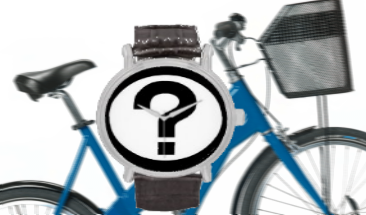
\includegraphics[width=0.8\linewidth]{graphics/biketime}
\end{center}

\end{frame}

\subsection{Modeling the system}

\begin{frame}{Simple hotspot model}
\begin{figure}[H]
\begin{tikzpicture}[->,>=stealth',shorten >=1pt,auto,node distance=10cm,
  thick,main node/.style={circle,fill=blue!20,draw,font=\sffamily\Large\bfseries}]

  \node[main node] (1) {$H_1$};
  \node[main node] (2) [right of=1] {$H_2$};

  \path[every node/.style={font=\sffamily\small}]
    (1) edge [bend left] node {0.3} (2)
        edge [loop left] node {0.7} (1)
    (2) edge [bend left] node {0.6} (1)
        edge [loop right] node {0.4} (2);
\end{tikzpicture}
\caption{A Markov chain model of a system with two bike hotspots}
\label{markov:model:simple}
\end{figure}
\end{frame}

\begin{frame}
\begin{center}
Where do we place the black bike?	
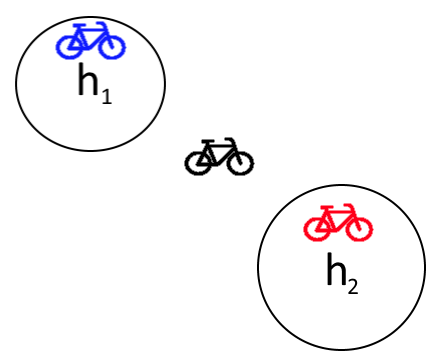
\includegraphics[scale=0.7]{graphics/world}
\end{center}
\end{frame}

\begin{frame}{Departure state model}
\begin{figure}[H]
\begin{tikzpicture}[->,>=stealth',shorten >=1pt,auto,node distance=4cm,
  thick,main node/.style={circle,fill=blue!20,draw,font=\sffamily\Large\bfseries}]

  \node[main node] (B1) {$h_1$};
  \node[main node,font=\sffamily\small] (D1) [right = 2cm of B1] {$d_1$};
  \node[main node,font=\sffamily\small] (D2) [right of=D1] {$d_2$};
  \node[main node] (B2) [right = 2cm of D2] {$h_2$};

  \path[every node/.style={font=\sffamily\small}]
    (B1) edge [bend left] node {0.05} (B2)
         edge [loop left] node {0.65} (B1)
         edge [bend left] node[below] {0.3} (D1)
    (B2) edge [bend left] node {0.15} (B1)
         edge [loop right] node {0.35} (B2)
         edge [bend left] node[above] {0.5} (D2)
    (D1) edge [bend left] node[above] {0.1} (B1)
         edge [loop right] node {0.6} (D1)
         edge [bend left] node[below left] {0.3} (B2)
    (D2) edge [bend left] node[below] {0.1} (B2)
         edge [loop left] node {0.7} (D2)
         edge [bend left] node[above right] {0.2} (B1);
\end{tikzpicture}
\caption{A Markov chain model with two hotspots and departure states}
\label{markov:model:complex}
\end{figure}

% VISUALIZE
% http://setosa.io/blog/2014/07/26/markov-chains/index.html
%[[0.65,0.30,0.05,0.00],
%[0.10,0.60,0.30,0.00],
%[0.15,0.00,0.50,0.35],
%[0.20,0.00,0.10,0.70]
%]
\end{frame}

\subsection{Creating the model}

\begin{frame}{}
	
\begin{center}
We want to generate the model with data from the GPS receivers on the bikes
	
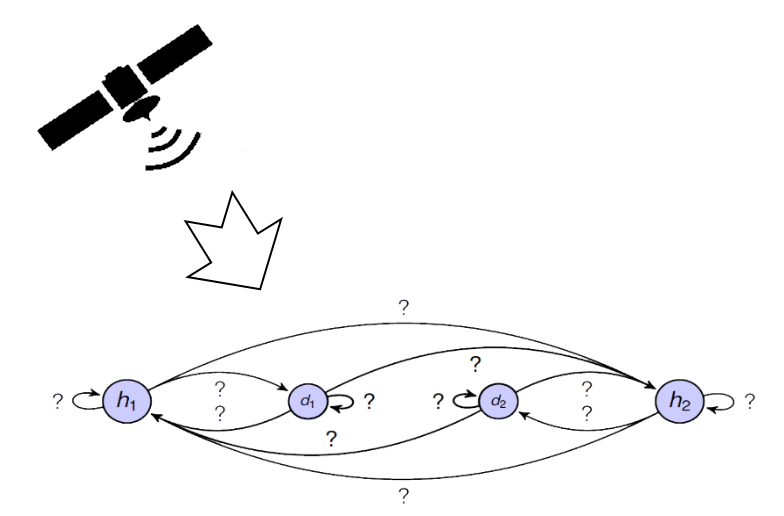
\includegraphics[width=0.8\linewidth]{graphics/build_the_model}
\end{center}

\end{frame}

\begin{frame}{The algorithm}
\def\HiLi{\leavevmode\rlap{\hbox to \hsize{\color{yellow!50}\leaders\hrule height .8\baselineskip depth .5ex\hfill}}}


\scalebox{0.8}{
	
\begin{algorithm}[H]
\SetAlgoNoEnd
\textbf{CreateModel}($H, G, step$)\\
Let $M$ be an empty $m \times m$ matrix with $m = 2|H|$ \\
\ForEach{$b \in B$}
	{
	$g \leftarrow G(b).first$\\
	$L(b) \leftarrow \textbf{NearestState}(H, g)$
	}
 Let $d \leftarrow G.first.date$\\
Let $l \leftarrow G.last.date$\\
\While{$d \leq l$}
	{
	\ForEach{$b \in B$}
		{
		$g \leftarrow G(b, d)$\\
		$n \leftarrow \textbf{NearestState}(H, g)$\\
		\If{$n \in D \wedge L(b) \in D$}
			{
		$n \leftarrow L(b)$
			}
		\ElseIf{$n \in D \wedge L(b) \in H$}
			{
			$n \leftarrow L(b).departure$
			}
\HiLi			$ increment(M,L(b),n) $\\
\HiLi			$ L(b) \leftarrow n $
		}
	$d \leftarrow \text{Add}(d, step)$
	}
Normalize $M$\\
\Return{M}
\end{algorithm}

}
\end{frame}

\subsection{Predicting with the model}

\begin{frame}{}
	
\begin{center}
The initial distribution of bikes in the system

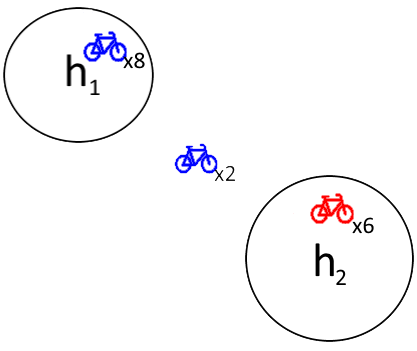
\includegraphics[scale=0.7]{graphics/initialworld}
	
$ (8,2,6,0) $
\end{center}
\end{frame}

\begin{frame}
	
\begin{center}	
	
$ P_i \times \tau_M = P_{i+1}$\\
		
		
$$
(8, 2, 6, 0)
\begin{bmatrix}
0.65 & 0.3 & 0.05 & 0\\
0.1  & 0.6 & 0.3  & 0\\
0.15 & 0   & 0.35 & 0.5\\
0.2  & 0   & 0.1  & 0.7
\end{bmatrix}
=
(6.3, 3.6, 3.1, 3)
$$
\end{center}
\end{frame}
